\documentclass[12pt,a4paper]{article}
\usepackage[utf8]{inputenc}
\usepackage[T1]{fontenc}
\usepackage{amsmath}
\usepackage{amsfonts}
\usepackage{amssymb}
\usepackage{multicol}
\usepackage{qrcode}
\usepackage{lmodern}
\usepackage{colortbl}%permet de griser les cases
\usepackage{tabularx, multirow}
%\usepackage{lscape}
\usepackage{xcolor}
%\usepackage{graphicx}
\usepackage{tikz,tkz-base}
\input{preambulemanu.sty}
\usepackage[left=2cm,right=2cm,top=2cm,bottom=2cm]{geometry}
\def\Oij{$\left(\text{O},~\vec{i},~\vec{j}\right)$}
\usepackage{fancyhdr}
\usepackage{MnSymbol,wasysym}

%Permet le code python sur lateX
\usepackage{minted}
\usemintedstyle{lovelace}



\begin{document}
\textbf{2nd} \hfill \textbf{Fonctions affines} \hfill Lycée Jean Rostand\\
\trait 

\subsection*{Exercice 1}

Parmi les fonctions suivantes définies sur $\R$, dire lesquelles sont affines. Justifier la réponse.

\begin{enumerate}
\begin{minipage}[t]{0.4\linewidth}
\item $f(x)=\sqrt{2}x+1$
\item $g(x)=\dfrac{2}{3x}+1$
\end{minipage}
\begin{minipage}[t]{0.4\linewidth}
\item $h(x)=5(x+1)$
\item $i(x)=-3x$
\end{minipage}
\begin{minipage}[t]{0.4\linewidth}
\item $j(x)=2x^2+3$
\item $k(x)=(x+1)^2-x^2$
\end{minipage}
\begin{minipage}[t]{0.4\linewidth}
\item $l(x)=4$

\end{minipage}
\end{enumerate}

\subsection*{Exercice 2}
Les expressions suivantes définissent-elles une fonction affine ? (justifier et, si oui, préciser le coefficient directeur) :\medskip\\
$f(x)=-5x^2+7x-1$\hfill $g(x)=\frac{3x-5}{7}$\hfill $h(x)=(x-3)(2x-5)-2x^2$
\subsection*{Exercice 3}

Dans un même repère \Oij{}, tracer la courbe représentative de chacune des fonctions suivantes définies sur $\R$.


\begin{enumerate}
\begin{minipage}[c]{0.3\linewidth}
\item $f(x)=2x-3$
\end{minipage}
\begin{minipage}[c]{0.3\linewidth}
\item $g(x)=-x+4$
\end{minipage}
\begin{minipage}[c]{0.3\linewidth}
\item $h(x)=\dfrac{1}{2}x-2$
\end{minipage}
\begin{minipage}[c]{0.3\linewidth}
\item $i(x)=-3x$

\end{minipage}
\end{enumerate}


\subsection*{Exercice 4}

\begin{enumerate}
    \item Dans un même repère, représenter les fonctions $f$ et $g$ définie sur $\R$ par $f(x)=-2x+5$ et $g(x)=\dfrac{1}{2}x$
    \item Résoudre graphiquement puis par le calcul l'équation $f(x)=g(x)$
\end{enumerate}

\subsection*{Exercice 5}

\begin{enumerate}
    \item Déterminer graphiquement l'expression de la fonction de affine $f_1$ dont la représentation graphique est la droite $\mathscr{D}{_1}$
    \item Déterminer graphiquement l'expression de la fonction de affine $f_2$ dont la représentation graphique est la droite $\mathscr{D}{_2}$
    \item Tracer la droite qui représente la fonction affine $f_3$ définie par $f_3(x)=-\dfrac{5}{4}x+4$.
    \item Déterminer par le calcul l'expression de la fonction affine $f_4$ dont la représentation graphique est la droite $(EF)$ avec $E(-1;-3)$ et $F(1;1)$.
\end{enumerate}



\begin{center}
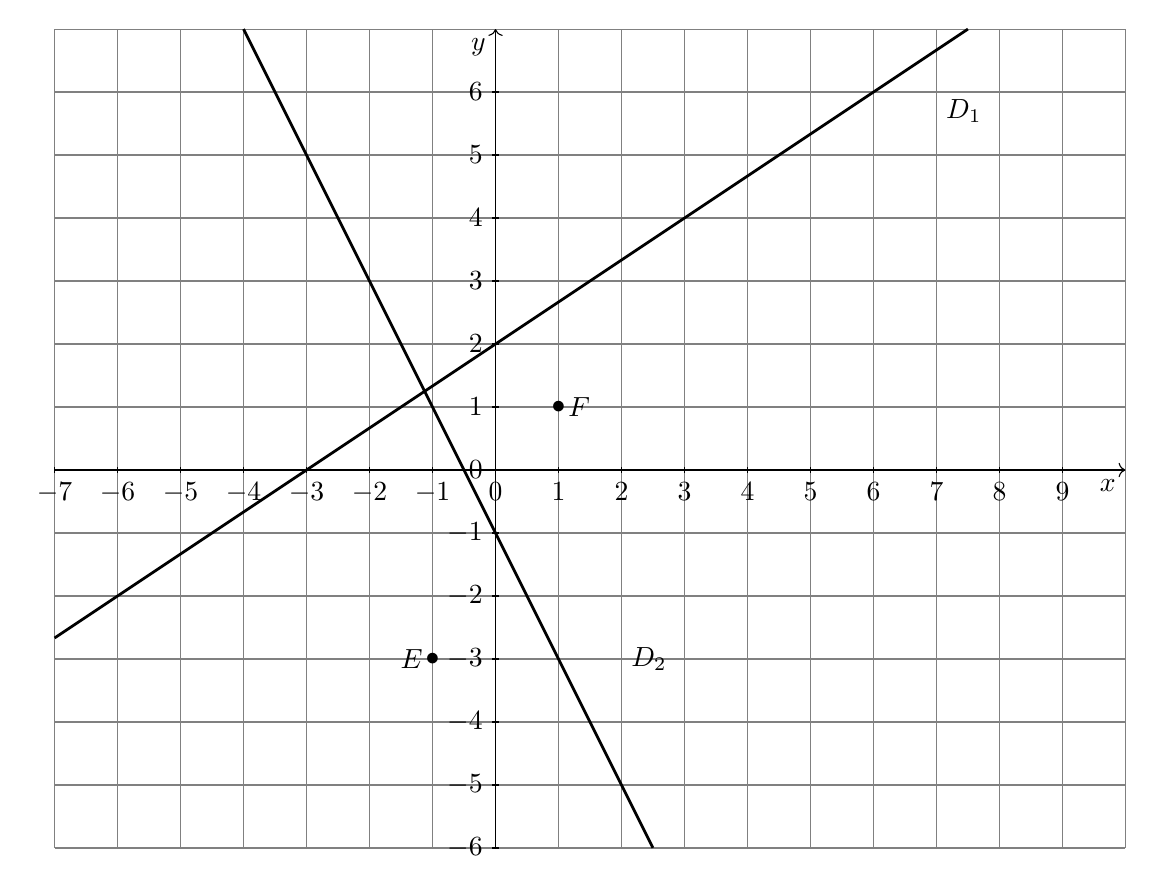
\begin{tikzpicture}[scale=0.8]

\draw [gray,xstep=1,ystep=1] (-7,-6) grid (10,7);
\draw [->] (-7,0) -- (10,0) node [below left] {$x$};
\draw [->] (0,-6) -- (0,7) node [below left] {$y$};

\foreach \x in {-7,...,9}
\draw (\x,0.5mm) -- (\x,-0.5mm) node [below] {$\x$};
\foreach \y in {-6,...,6}
\draw (0.5mm,\y) -- (-0.5mm,\y) node [left] {$\y$};


\draw [domain=-7:7.5,line width=1pt,samples=100] plot (\x,{2/3*\x+2});
\draw [domain=-4:2.5,line width=1pt,samples=100] plot (\x,{-2*\x-1});
\draw (7,5.7) node [right] {$\mathscr{D}_{1}$};
\draw (2,-3) node [right] {$\mathscr{D}_{2}$};

\draw (-1,-3) node{$\bullet$};
\draw (-1,-3) node[left]{$E$};
\draw (1,1) node{$\bullet$};
\draw (1,1) node[right]{$F$};

\end{tikzpicture}
\end{center}











\subsection*{Exercice 6}
\begin{enumerate}
\item Construire, dans le repère de la question /2, les représentations graphiques des fonctions définies par $f(x)=3x-2$, $g(x)=-\frac{3}{4}x+5$, $h(x)=-3$ et $k(x)=2x$.
\item Donner l'expression de chaque fonction associée aux droites suivantes:\\
\end{enumerate}
\begin{center}
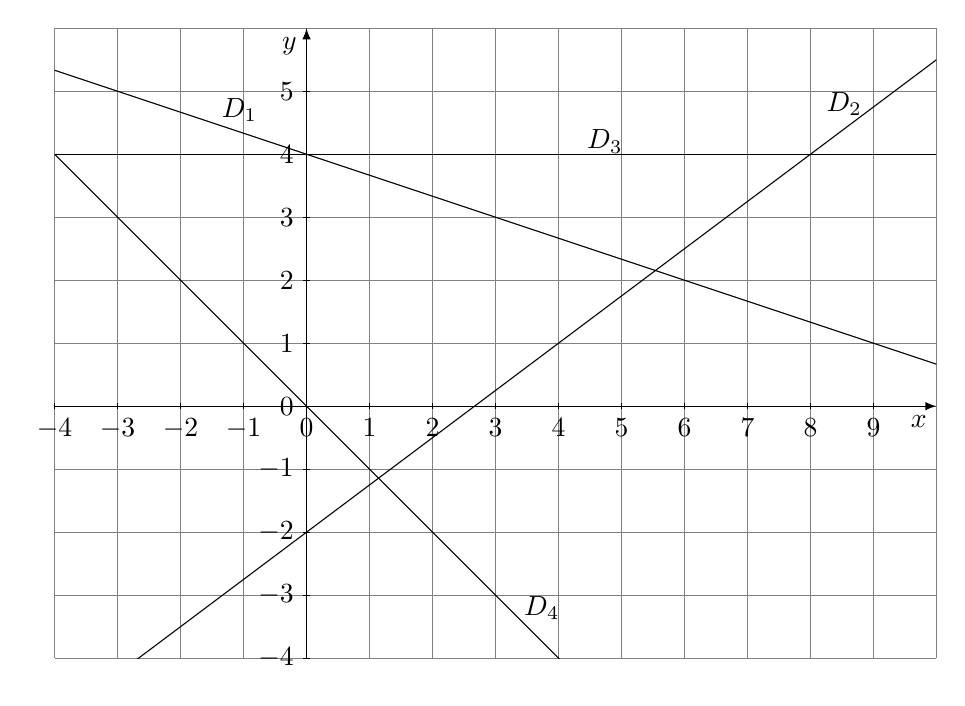
\begin{tikzpicture}[scale=0.8]
\draw [gray,xstep=1,ystep=1] (-4,-4) grid (10,6);
\draw [->,>=latex] (-4,0) -- (10,0) node [below left] {$x$};
\draw [->,>=latex] (0,-4) -- (0,6) node [below left] {$y$};

\foreach \x in {-4,...,9}
\draw (\x,0.5mm) -- (\x,-0.5mm) node [below] {$\x$};
\foreach \y in {-4,...,5}
\draw (0.5mm,\y) -- (-0.5mm,\y) node [left] {$\y$};

%\draw (0,0) node [below left] {$O$};

\clip (-4,-4) rectangle (10,6);
\draw [domain=-4:10,samples=100] plot (\x,{-(1/3)*\x+4});
\draw [domain=-4:10,samples=100] plot (\x,{-1*\x});
\draw [domain=-4:10,samples=100] plot (\x,{(3/4)*\x-2});
\draw [domain=-4:10,samples=100] plot (\x,{4});
\draw (-1.5,4.7) node [right] {$\mathscr{D}_{1}$};
\draw (8.1,4.8) node [right] {$\mathscr{D}_{2}$};
\draw (4.3,4.2) node [right] {$\mathscr{D}_{3}$};
\draw (3.3,-3.2) node [right] {$\mathscr{D}_{4}$};
\end{tikzpicture}
\end{center}

\subsection*{Exercice 7}
Déterminer l'expression de la fonction affine $f$ telle que $f(-2)=4$ et $f(5)=7$.

\subsection*{Exercice 8}

On sait que $f$ est une fonction affine.\\
Dans chacun des cas et lorsque cela est possible, exprimer $f(x)$ en fonction de $x$

\begin{enumerate}
\begin{minipage}[c]{0.4\linewidth}
\item $f(-2)=-1$ et $f(4)=2$
\item $f(-1)=5$ et $f(-2)=1$
\end{minipage}
\begin{minipage}[c]{0.4\linewidth}
\item $f(6)=4$ et $f(-9)=-6$
\item $f(-1)=2$ et $f(3)=2$
\end{minipage}
\begin{minipage}[c]{0.4\linewidth}
\item $f(1)=\dfrac{1}{2}$ et $f\left(\dfrac{3}{2}\right)=-\dfrac{1}{2}$
\item $f(1)=-1$ et $f(1)=2$
\end{minipage}
\end{enumerate}

\subsection*{Exercice 9}

D'après ce tableau de valeurs, la fonction $g$, définie sur $\R$, peut-elle être une fonction affine ?

\begin{center}
 { \setlength{\tabcolsep}{9mm}
\begin{tabular}{|c|c|c|c|c|} \hline
$x$ & $1$&$3$& $3,5$&$4,5$ \\ \hline
$g(x)$ &$-5$ & $-1$&$0$&$3$  \\ \hline
\end{tabular} }
   
\end{center}

\subsection*{Exercice 10}
Dans chacun des cas suivants établir le tableau de signes de la fonction $f$.

\begin{enumerate}
\begin{minipage}[c]{0.4\linewidth}
\item $f(x)=2x-4$
\item $f(x)=-3x+2$
\end{minipage}
\begin{minipage}[c]{0.4\linewidth}
\item $f(x)=4x$
\item $f(x)=-5x+7$
\end{minipage}
\begin{minipage}[c]{0.4\linewidth}
\item $f(x)=3x+4$ 
\item $f(x)=-7$
\end{minipage}
\end{enumerate}


\subsection*{Exercice 11}
Soient $f$ et $g$ les fonctions définies par $f(x)=5x-2$ et $g(x)=\frac{5}{3}x+6$.\medskip
\begin{enumerate}
\item Résoudre l'équation $f(x)=g(x)$. En déduire le point d'intersection entre les courbes $C_{f}$ et $C_{g}$.\medskip
\item Le point de coordonnées $(2;7)$ se trouve-t-il sur la courbe de $f$ ?\medskip 
\end{enumerate}

\subsection*{Exercice 12}

Dresser le tableau de signes des expressions suivantes:
\begin{enumerate}
    \item $A(x)=x+7$
    \item $B(x)=5-x$
\end{enumerate}


\subsection*{Exercice 13}

Dresser le tableau de signes des expressions suivantes:
\begin{enumerate}
    \item $A(x)=3x+4$
    \item $B(x)=-5x+8$
\end{enumerate}

\subsection*{Exercice 14}

\begin{enumerate}
    \item Etudier le signe des expressions $A(x)=4x-12$ et $B(x)=-3x+7$
    \item En déduire le signe du produit $A(x)\x B(x)$
    
\end{enumerate}

\subsection*{Exercice 15}

Dresser le tableau de signes des expressions suivantes:
\begin{enumerate}
    \item $A(x)=(x+4)(2x-3)$
    \item $B(x)=(6-x)(x-3)$
\end{enumerate}



\subsection*{Exercice 16}

\begin{enumerate}
    \item Etudier le signe des expressions $A(x)=2-x$ et $B(x)=4x-3$
    \item En déduire le signe du produit $\dfrac{A(x)}{ B(x)}$
    
\end{enumerate}

\subsection*{Exercice 17}

Dresser le tableau de signes des expressions suivantes:
\begin{enumerate}
    \item $A(x)=\dfrac{6x-4}{2-3x}$
    \item $B(x)=\dfrac{3x+2}{5x-1}$
\end{enumerate}



\subsection*{Exercice 18}
\begin{enumerate}
\item Construire le tableau de signe du produit $(2x-4)(-3x-5)$.\medskip
\item Construire le tableau de signe du quotient $\frac{-3x+9}{7x-5}$.\medskip
\item Donner l'ensemble des solutions de l'inéquation $(2x-4)(-3x-5)<0$ grâce à la réponse à 1/.\medskip
\item Résoudre l'inéquation $\frac{-3x+9}{7x-5}\geqslant0$ grâce à 2/
\end{enumerate}



\subsection*{Exercice 19}

Dans un repère \Oij{}, on considère les points $A(-1;1)$, $B(2;2)$, $C(0;2)$ et $D(3;1)$.\\
On appelle $f$ la fonction affine dont la représentation graphique est la droite $(AB)$ et $g$ la fonction affine dont représentation graphique est la droite $(CD)$. On note $I$ le point d'intersection des droites $(AB)$ et$(CD)$.

\begin{enumerate}
    \item Placer les points $A$, $B$, $C$ et $D$ dans le repère \Oij{} puis tracer les droites $(AB)$ et $(CD)$
    \item Déterminer graphiquement une valeur approchée des coordonnées du point $I$
    \item Exprimer $f(x)$ en fonction de $x$ puis $g(x)$ en fonction de $x$
    \item Déterminer les coordonnées exactes de $I$
\end{enumerate}
\newpage
\subsection*{Exercice 20}

Deux chauffeurs de taxi pratiquent des tarifs  différents:

\begin{itemize}
    \item \textbf{Tarif A}: $5$ \EUR{} de prise en charge et $0,4$ \EUR{} par kilomètre parcouru.
    \item  \textbf{Tarif B}: Pas de frais de prise en charge et $0,6$ \EUR{} par kilomètre parcouru.
\end{itemize}

On désigne respectivement $A(x)$ et $ B(x)$ le prix payé en euros auprès des taxis $A$ et $B$ pour un nombre $x$ de kilomètres parcourus. \\
Dans le repère ci-dessous, on a représenté graphiquement les fonctions $x\mapsto A(x)$ et $x\mapsto B(x)$ pour $0\leq x\leq 40$



\begin{center}
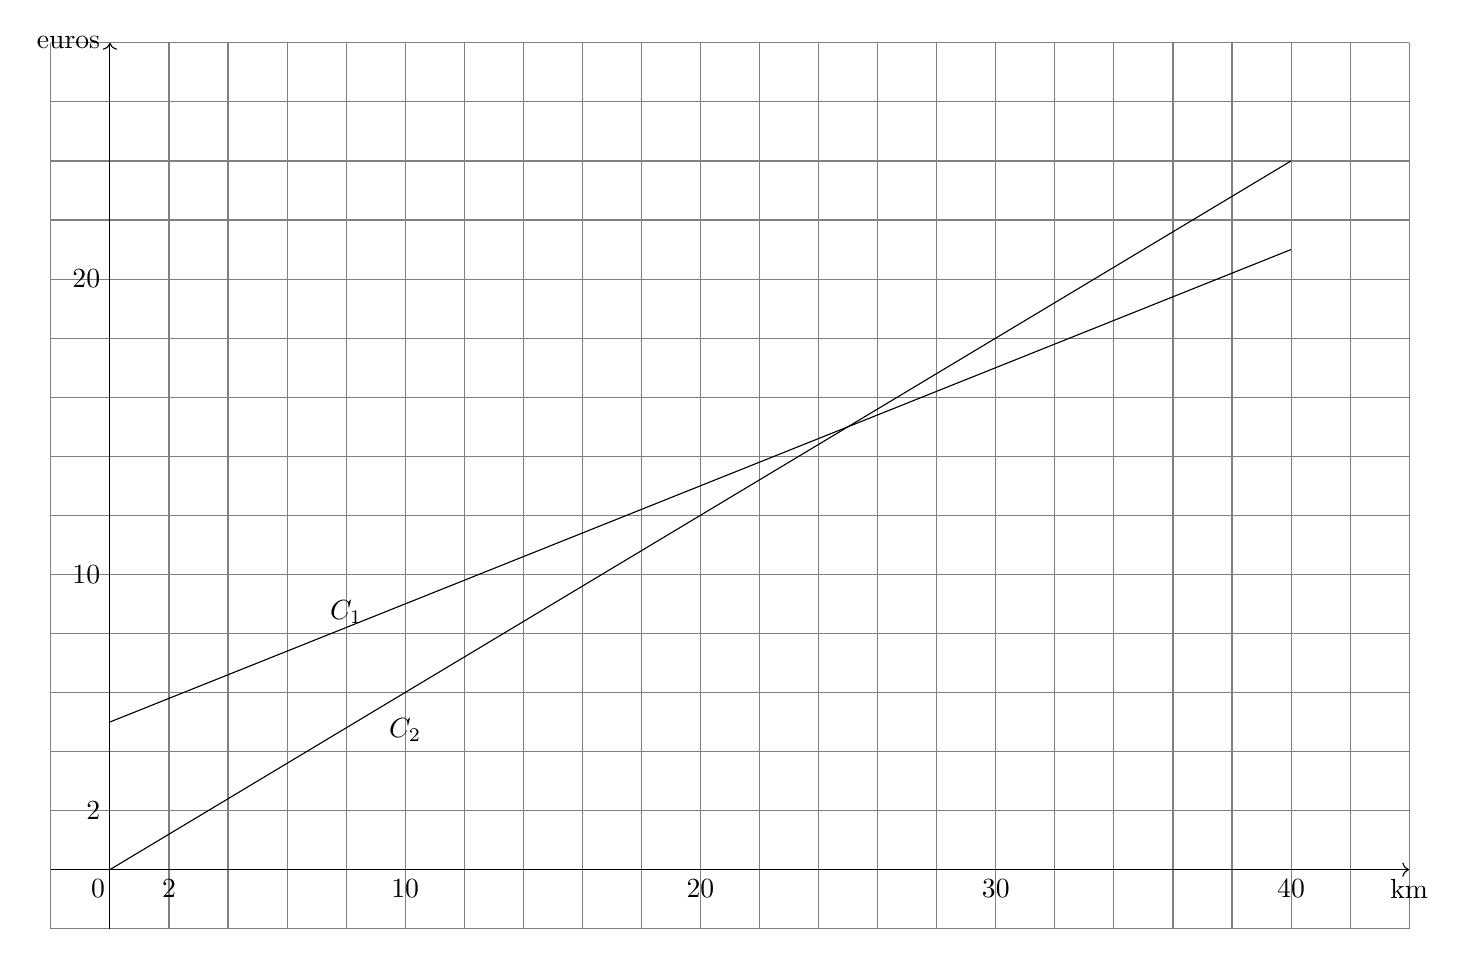
\begin{tikzpicture}[scale=0.75]
\draw [gray,xstep=1,ystep=1] (-1,-1) grid (22,14);
\draw [->] (-1,0) -- (22,0) node [below] {km};
\draw [->] (0,-1) -- (0,14) node [left] {euros};

\draw (-0.2,0) node[left,below]{$0$};
\draw (1,0) node[below]{$2$};
\draw (5,0) node[below]{$10$};
\draw (10,0) node[below]{$20$};
\draw (15,0) node[below]{$30$};
\draw (20,0) node[below]{$40$};
\draw (0,1) node[left]{$2$};
\draw (0,5) node[left]{$10$};
\draw (0,10) node[left]{$20$};
\draw[domain=0:20] plot(\x,{0.6*(\x)} );
\draw[domain=0:20] plot(\x,{0.4*(\x)+2.5} );
\draw (4,4) node [above] {$\mathscr{C}_{1}$};
\draw (5,2) node [above] {$\mathscr{C}_{2}$};
\end{tikzpicture}
\end{center}

\begin{enumerate}
    \item Associer chacune des courbes $\mathscr{C}_{1}$ et $\mathscr{C}_{2}$ aux tarifs pratiqués par les taxis.
    \item Quel est le taxi le plus économique lorsque l'on désire faire un parcours de 20km ? de 30 km?
    \item Exprimer $A(x)$ et $B(x)$ en fonction de $x$.
    \item Un troisième taxi fait payer $11,50$\EUR{} pour $17$ km parcourus et $20,50$\EUR{} pour $35$ km.\\ Le prix d'un parcours est une fonction affine du nombre de kilomètres parcourus. \\ Déterminer le prix d'un parcours de $30 $ km avec ce taxi.
\end{enumerate}



\end{document}
 